\documentclass[10pt,twocolumn,letterpaper]{article}
\usepackage[pagenumbers]{cvpr}
\usepackage{amsmath,amssymb}
\usepackage{booktabs,multirow}
\usepackage{graphicx}
\usepackage{microtype}
\usepackage{siunitx}
\usepackage{algorithm}
\usepackage{algpseudocode}
\usepackage{enumitem}
\usepackage{xspace}
\usepackage{balance}
\newcommand{\method}{PV-SRA-3DGS\xspace}
\newcommand{\ours}{pressure-triggered preservation\xspace}
\DeclareMathOperator*{\argmax}{arg\,max}
\setlength{\abovecaptionskip}{3pt}
\setlength{\belowcaptionskip}{-2pt}
\setlist[itemize]{leftmargin=*,nosep}

\definecolor{cvprblue}{rgb}{0.21,0.49,0.74}
\usepackage[breaklinks,colorlinks,allcolors=cvprblue]{hyperref}
\def\confName{CVPR}\def\confYear{2027}
\title{Supplementary Material: Peak-VRAM-Constrained Spatial Resource Allocation with Pressure-Triggered Preservation for 3D Gaussian Splatting}
\author{Anonymous CVPR submission}
\begin{document}\maketitle
\section{Allocator Telemetry}
\begin{figure*}[h]
\centering
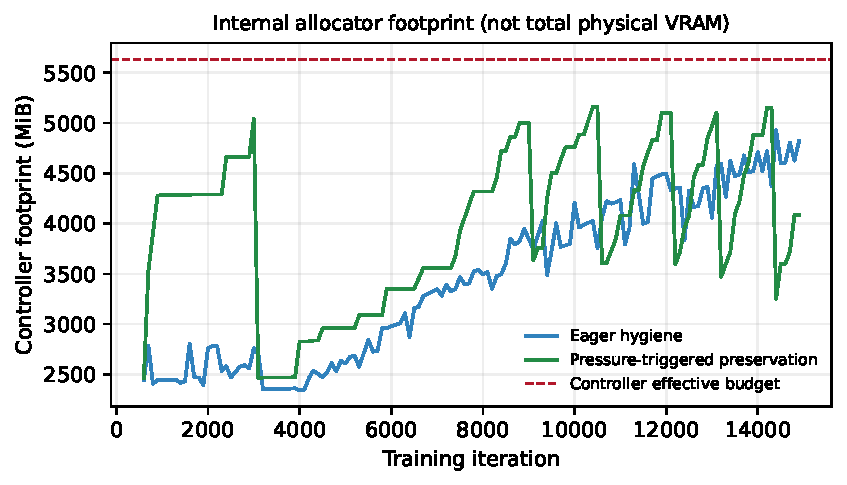
\includegraphics[width=.85\textwidth]{../figures/fig6_memory_trace.pdf}
\caption{Internal conservative allocator footprint on Bonsai seed 0. This is $\max(A_t,R_t)+B_{\rm np}$ and must not be interpreted as whole-device VRAM. The red line is the controller's effective 5,632-MiB budget.}
\end{figure*}
\section{Evidence Scope}
Every quantitative statement is mapped to a raw evaluation JSON, PLY header, benchmark verification file, calibration file, or a deterministic recomputation in \texttt{quantitative\_claims.csv}. The verifier inspects all 24 physical run directories and refuses to generate figures when raw results and the canonical registry disagree.
\end{document}
